\documentclass{article}
\usepackage[left=3cm,right=3cm,top=3cm,bottom=3cm]{geometry}
\usepackage{amsmath,amssymb,amsthm,pgfplots,tikz}
\usetikzlibrary{patterns}
\usepackage{color}
\setlength{\parindent}{2mm}
\newcommand{\TODO}[1]{\textcolor{red}{TODO: #1}}

\begin{document}
\title{Geometry and Topology: Homework 1}
\author{Li Ling Ko\\ lko@nd.edu}
\date{\today}
\maketitle

\begin{enumerate}
  \item
    \begin{proof}
      We first prove the forward implication. Fix $\epsilon>0$ and $p\in X$.
      By assumption, the set $U=f^{-1}(B_\epsilon(f(p)))\subseteq X$ is open.
      By choice of $U$, it must contain $p$. Then there must exist
      some $\delta>0$ such that the $d_Y$ ball $B_\delta(p)$ is contained in
      $U$. This $\delta$ satisfies the requirement. \\

      For the converse, assume the second definition. Let $U\subseteq Y$ be
      open, and $x\in f^{-1}(U)$. We want to find an open set in $f^{-1}(U)$
      that contains $x$. Since $U$ is open, $f(x)$ must be contained in a
      ball $B_\epsilon(f(x))\subseteq U$ for some $\epsilon>0$. Let $\delta$
      be the one given by the assumption. Then $B_\delta(x)$ satisfies the
      requirements for the open set we need.
    \end{proof}
  \item
    \begin{proof}
      Since $\pi':X\rightarrow Y'$ is a continuous function such that
      $\pi'(p)\sim\pi'(q)$ for all $p,q\in X$ satisfying $p\sim q$, we can
      replace the role of $Z$ by $Y'$ in the first set of properties, and
      get a continuous function $\vec{f}:Y\rightarrow Y'$ such that
      $\pi'=\vec{f}\circ\pi$. By symmetrical argument, there is also a
      continuous function $\vec{f'}:Y'\rightarrow Y$ such that
      $\pi=\vec{f'}\circ\pi'$. We show that
      $\vec{f}\circ\vec{f'}=\text{id}$, and
      $\vec{f'}\circ\vec{f}=\text{id}$. It suffices to prove the first
      equality since the argument for the second equality will be
      symmetrical. Let $\pi(x)\in Y$. By uniqueness of $\vec{f}$, $\vec{f}$
      must send $\pi(x)$ to $\pi'(x)$. Then by uniqueness of $\vec{f'}$,
      $\vec{f'}$ must send $\pi'(x)$ back to $\pi(x)$. Hence
      $\vec{f}\circ\vec{f'}=\text{id}$.
    \end{proof}
  \item
    \begin{enumerate}
      \item
        \begin{proof}
          We show that $\mathbb{R}^2/\sim$ is homeomorphic to the real line
          $\mathbb{R}$, by proving that the map
          $f:\mathbb{R}^2/\sim\rightarrow\mathbb{R}$ defined by
          $[(r,0)]\mapsto r$ is a homeomorphism. \\

          We first show that this map is well-defined. The equivalence
          class $[(r,0)]$ comprises all solutions to the quadratic curve
          $x+y^2=r$. So if $r_1\neq r_2\in\mathbb{R}$, then $(r_1,0)$ and
          $(r_2,0)$ belong to distinct equivalence classes. Also, every
          $(a,b)\in\mathbb{R}^2$ belongs to class $[(a+b^2,0)]$. Hence, map
          $f$ is well-defined. \\

          Map $f$ is clearly bijective, with inverse $f^{-1}$ defined by
          $f^{-1}(r)=[(r,0)]$. It remains to show that $f$ and $f^{-1}$ are
          continuous. We first show that $f$ is continuous. Given an open
          interval $(r_1,r_2)\in\mathbb{R}$, we need to show that its
          pre-image $\{[(r,0)]:r_1<r<r_2\}$ is open in $\mathbb{R}^2/\sim$.
          This is the same as showing that $\{(x,y):r_1<x+y^2<r_2\}$ is
          open in $\mathbb{R}^2$, which is true. \\

          Finally, we show that $f^{-1}$ is continuous, which is equivalent
          to showing that $f$ sends open sets to open sets. Let
          $\bar{U}=\{[(r_i,0)]:i\in I\}$ be an open set in
          $\mathbb{R}^2/\sim$. Then $f(U)=\{r_i:i\in I\}$. Let $r\in f(U)$.
          We want to show that there is an open interval
          $B_\epsilon(r)\subset\mathbb{R}$ that is contained in $f(U)$.
          Since $\bar{U}$ is open in $\mathbb{R}^2/\sim$,
          $U=\{(x,y):x+y^2\in\{r_i:i\in I\}\}$ must be open in
          $\mathbb{R}^2$. Also, $(r,0)\in U$, so there must be a ball
          $B_\epsilon((r,0))\subset\mathbb{R}^2$ containing $(r,0)$ in $U$.
          The image of this ball under $f$ is an open interval
          $B_\epsilon(r)\subset\mathbb{R}$ that is contained in $f(U)$ and
          that contains $r$, which is the interval we are looking for.
        \end{proof}
      \item
        \begin{proof}
          We show that $\mathbb{R}^2/\sim$ is homeomorphic to the half real
          line $R=\mathbb{R}^+\cup\{0\}$, by proving that the map
          $f:\mathbb{R}^2/\sim\rightarrow R$ defined by
          $[(r,0)]\mapsto |r|$ is a homeomorphism. \\

          We first show that this map is well-defined. The equivalence
          class $[(r,0)]$ comprises all solutions to the circle
          $x^2+y^2=r^2$. So if $r_1\neq r_2\in\mathbb{R}$, then $(r_1,0)$
          and $(r_2,0)$ belong to distinct equivalence classes. Also, every
          $(a,b)\in\mathbb{R}^2$ belongs to class $[(a^2+b^2,0)]$. Hence,
          map $f$ is well-defined. \\

          Map $f$ is clearly bijective, with inverse $f^{-1}$ defined by
          $f^{-1}(r)=[(r,0)]$. It remains to show that $f$ and $f^{-1}$ are
          continuous. We first show that $f$ is continuous. Given an open
          interval $(r_1,r_2)\in R$ (or $(0,r_2)\in R$), we need to show
          that its pre-image $\{[(r,0)]:r_1<r<r_2\}$ (or $\{[(r,0)]:0\leq
          r<r_2\}$) is open in $R$. This is the same as showing that
          $\{(x,y):r_1<x^2+y^2<r_2\}$ (or $\{(x,y):x^2+y^2<r_2\}$) is open
          in $\mathbb{R}^2$, which is true. \\

          Finally, we show that $f^{-1}$ is continuous, which is equivalent
          to showing that $f$ sends open sets to open sets. Let
          $\bar{U}=\{[(r_i,0)]:i\in I\}$ be an open set in
          $\mathbb{R}^2/\sim$. Then $f(U)=\{|r_i|:i\in I\}$. Let $r\in f(U)$.
          We want to show that there is an open interval
          $B_\epsilon(r)\subset R$ that is contained in $f(U)$.
          Since $\bar{U}$ is open in $\mathbb{R}^2/\sim$,
          $U=\{(x,y):x^2+y^2\in\{r_i^2:i\in I\}\}$ must be open in
          $\mathbb{R}^2$. Also, $(r,0)\in U$, so there must be a ball
          $B_\epsilon((r,0))\subset\mathbb{R}^2$ containing $(r,0)$ in $U$.
          The image of this ball under $f$ is an open interval
          $B_\epsilon(r)\subset\mathbb{R}$ that is contained in $f(U)$ and
          that contains $r$, which is the interval we are looking for.
        \end{proof}
    \end{enumerate}
  \item
    \begin{enumerate}
      \item
        \begin{proof}
          Curves of the form $(x^2-1)e^y=c$ can be reduced to curves of the
          form $y=c-ln(1-x^2)$. We vary $c$ across $\mathbb{R}$ to get a
          series of U-shaped curves that are symmetric about the $y$-axis
          and that are $y$-translations of each other. Every $(a,b)$ in
          $(-1,1)\times\mathbb{R}$ belongs to the equivalence class
          $[(0,b+ln(1-a^2))]$. Hence the equivalence classes of the points
          where $x\neq\pm1$ is homeomorphic to $\mathbb{R}$. For the line
          $x=1$, its equivalence class is disjoint from the equivalence
          classes of any other point with $x$-coordinate not equal to 1 or
          -1, because $y=c-ln(x^2-1)$ does not have solutions with $x=\pm
          1$. The same can be said for the line $x=-1$. Hence in $X/\sim$,
          the lines $x=-1$ and $x=1$ are reduced to distinct points. The
          equivalence classes are shown in the diagram below. \\

          \begin{center}
            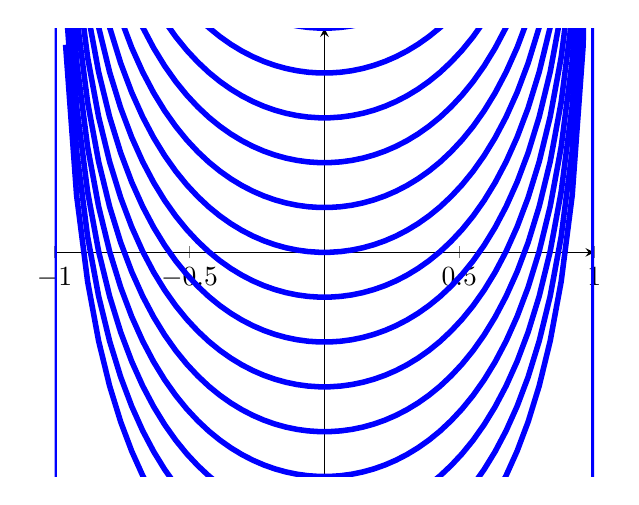
\begin{tikzpicture}
              \begin{axis}[
                xtick=\empty,xmin=-1,xmax=1,
                ytick=\empty,ymin=-1,ymax=1,
                xtick={-1.0,-0.5,0.0,0.5,1.0},
                axis lines=middle,
                ]
                \addplot[draw,blue,domain=-1:1,line width=2pt] coordinates{(-1,-1)(-1,1)};
                \addplot[draw,blue,domain=-1:1,line width=2pt] coordinates{(1,-1)(1,1)};
                \addplot[draw,blue,domain=-1:1,samples=50,line width=2pt] plot{ 1.0-ln(1-x^2)};
                \addplot[draw,blue,domain=-1:1,samples=50,line width=2pt] plot{ 0.8-ln(1-x^2)};
                \addplot[draw,blue,domain=-1:1,samples=50,line width=2pt] plot{ 0.6-ln(1-x^2)};
                \addplot[draw,blue,domain=-1:1,samples=50,line width=2pt] plot{ 0.4-ln(1-x^2)};
                \addplot[draw,blue,domain=-1:1,samples=50,line width=2pt] plot{ 0.2-ln(1-x^2)};
                \addplot[draw,blue,domain=-1:1,samples=50,line width=2pt] plot{ 0.0-ln(1-x^2)};
                \addplot[draw,blue,domain=-1:1,samples=50,line width=2pt] plot{-0.2-ln(1-x^2)};
                \addplot[draw,blue,domain=-1:1,samples=50,line width=2pt] plot{-0.4-ln(1-x^2)};
                \addplot[draw,blue,domain=-1:1,samples=50,line width=2pt] plot{-0.6-ln(1-x^2)};
                \addplot[draw,blue,domain=-1:1,samples=50,line width=2pt] plot{-0.8-ln(1-x^2)};
                \addplot[draw,blue,domain=-1:1,samples=50,line width=2pt] plot{-1.0-ln(1-x^2)};
                \addplot[draw,blue,domain=-1:1,samples=50,line width=2pt] plot{-1.2-ln(1-x^2)};
                \addplot[draw,blue,domain=-1:1,samples=50,line width=2pt] plot{-1.4-ln(1-x^2)};
                \addplot[draw,blue,domain=-1:1,samples=50,line width=2pt] plot{-1.6-ln(1-x^2)};
              \end{axis}
            \end{tikzpicture}
          \end{center}
        \end{proof}
      \item
        \begin{proof}
          Denote the unique quotient map that sends $X$ to its quotient
          space $X/\sim$ by $\pi:X\rightarrow X/\sim$. \\

          Consider the distinct points $[(-1,0)]$ and $[(1,0)]$ in
          $X/\sim$. Let $\bar{U}$ and $\bar{V}$ be open sets covering the
          distinct points respectively. Without loss of generality, we can
          assume that the inverse quotient image $U=\pi^{-1}(\bar(U))$ and
          $V=\pi^{-1}(\bar(V))$ of these open sets include the balls
          $B_{r}((-1,0))$ and $B_{r_2}((-1,0))$ respectively, where $r<1$.
          Hence, $U$ and $V$ include the points $(-1+r/2,0)$ and $(1-r/2,0)$
          respectively. However, these two points belong to the same
          equivalence class and are therefore the same point in the
          quotient space, which implies that $\bar{U}$ and $\bar{V}$ cannot
          be disjoint in the quotient space.
        \end{proof}
    \end{enumerate}
  \item
    \begin{proof}
      We first use stereographic projection $p$ to map $S^n$ to
      $\mathbb{R}^n\cup\{\infty\}$. This map is known to be a continuous
      and bijective. Then, we map $\mathbb{R}^n\cup\{\infty\}$ to
      $\mathbb{D}^n$ using the scaled $\arctan$ function, which is also
      known to be continuous and bijective. The composition of these two
      maps is bijective and continuous since each individual map is
      bijective and continuous. To show that the inverse map is continuous,
      we use the fact that continuous bijections from Hausdorff to compact
      spaces are homeomorphisms.
    \end{proof}
  \item
    \begin{enumerate}
      \item
        \begin{proof}
          We prove the claim by induction on $n$. We prove a stronger
          claim by induction, that every point can be connected to either
          $x$ or $y$ by a piecewise linear path that does not intersect the
          image of $f$. \\

          In the base case, where $n=3$ and $f([0,1])$ draws a triangle, we
          can assume that $x$ is in the triangle and $y$ is outside the
          triangle. There are two cases to consider. In the first case, $p$
          is inside the triangle, and straight line from $p$ to $x$ will be
          the path we are looking for. In the second case, $p$ is outside
          the triangle, but we can always find a two-piece linear path to
          $y$ as illustrated in the diagram below. \\

          \begin{center}
            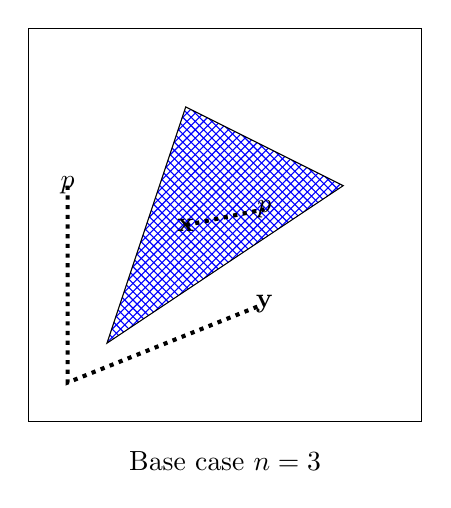
\begin{tikzpicture}
              %\draw[draw,domain=0:5] plot(\x,{\x});
              %\draw[help lines](0,0) grid(5,5);
              \path[draw,pattern=crosshatch,pattern color=blue] (1,1)--(2,4)--(4,3)--cycle;
              \path[draw,] (0,0)--(5,0)--(5,5)--(0,5)--cycle;
              \node[] at (2,2.5) {$\mathbf{x}$};
              \node[] at (3,2.7) {$p$};
              \path[draw,dotted,line width=1.5pt] (2,2.5)--(3,2.7);
              \node[] at (3,1.5) {$\mathbf{y}$};
              \node[] at (0.5,3) {$p$};
              \path[draw,dotted,line width=1.5pt] (0.5,3)--(0.5,0.5)--(3,1.5);
              \node[] at (2.5,-0.5) {Base case $n=3$};
            \end{tikzpicture}
          \end{center}

          Now we prove the inductive step. Assume we can find a piecewise
          linear path to either $x$ or $y$ for any $n$-gon. Consider the
          case of the $(n+1)$-gon. Every $(n+1)$-gon is a union of an
          $n$-gon and a non-overlapping triangle that shares exactly one
          side, as illustrated in the figure below, where the $n$-gon is
          shaded in cross pattern, the triangle is shaded in
          dotted pattern, and the shared edge is shown as a thick dashed
          line.
          \begin{center}
            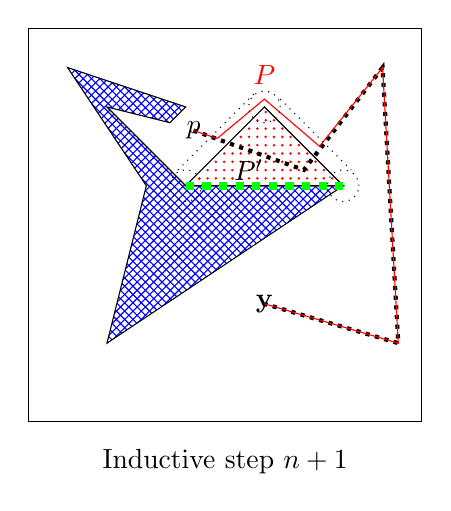
\begin{tikzpicture}
              %\draw[help lines](0,0) grid(5,5);
              \path[draw,pattern=crosshatch,pattern color=blue]
              (1,1)--(1.5,3)--(0.5,4.5)--(2,4)--(2,4)--(1.8,3.8)--(1,4)--(2,3)--(4,3)--cycle;
              \path[draw,pattern=dots,pattern color=red] (2,3)--(3,4)--(4,3)--cycle;
              \path[draw,] (0,0)--(5,0)--(5,5)--(0,5)--cycle;
              \node[] at (3,1.5) {$\mathbf{y}$};
              \node[] at (2.1,3.7) {$p$};
              \node[] at (2.8,3.2) {$P'$};
              \node[color=red] at (3.0,4.4) {$P$};
              \path[draw,dotted,line width=1.5pt]
              (2.1,3.7)--(3.5,3.2)--(4.5,4.5)--(4.7,1.0)--(3,1.5);
              \path[draw,color=red]
              (2.1,3.7)--(2.4,3.6)--(3.0,4.1)--(3.7,3.5)--(4.5,4.5)--(4.7,1.0)--(3,1.5);
              \node[] at (2.5,-0.5) {Inductive step $n+1$};
              \draw[dotted] (2,3) circle (0.2cm);
              \draw[dotted] (3,4) circle (0.2cm);
              \draw[dotted] (4,3) circle (0.2cm);
              \draw[draw,dotted] (1.9,3.2)--(2.9,4.2);
              \draw[draw,dotted] (3.2,4.1)--(4.1,3.2);
              \path[draw,line width=3pt,dashed,color=green] (2,3)--(4,3);
            \end{tikzpicture}
          \end{center}

          There are four cases to consider. In the first and easiest case,
          both $x$ and $p$ are in the $n$-gon. Then by induction, there is
          a piecewise linear path connecting them. In the second case, both
          $x$ and $p$ are in the $(n+1)$-gon, but one is in the triangle
          and the other is in the $n$-gon. Assume without loss of
          generality that $x$ is in the triangle. First draw a line from
          $x$ to the mid-point of the edge shared by both $n$-gon and
          triangle, then by induction using either the base case or the
          $n$-gon case there is a piecewise linear path from the mid-point
          to $p$. Finally, consider the case where $p$ lies outside the
          $(n+1)$-gon. If the path given by the $n$-gon case does not
          cut the new triangle, then we are done. Otherwise, we need to
          re-wire the original path near the triangle to ensure it does
          not cut the triangle. \\

          To re-wire the path, assume without loss of generality that the
          original path $P'$ enters the triangle from one of its non-shared
          edge and exits from the other non-shared edge, as illustrated in
          the diagram above. Before re-wiring the path, we find an open
          triangle-like cover of the triangle within which path $P'$ can be
          rewired across. To construct such a wrap, as illustrated in the
          diagram above, we consider smaller and smaller open balls around
          each vertex of the new triangle, such that each circle only
          intersects exactly two edges of the $(n+1)$-gon, and such that
          path $P'$ enters the wrap around the three circles before
          entering the triangle. Such circles exist because there are only
          a finite number of $(n+1)$-gon edges and vertices. Then can
          rewire path $P'$ to path $P$ to pass through the path given by
          the wrap without passing through the triangle, as illustrated
          above.
        \end{proof}
      \item
        \begin{proof}
          We first show that every point $p$ has a generic ray emanating
          from it. There are only a finite number of lines and a finite
          number of vertices $f(a_1),\ldots,f(a_k)$, so each point can only
          have a finite number of rays emanating from it that either
          intersects the image in infinite number of places (parallel to a
          line) or that passes through a vertex. However, the
          number of rays that can be emanated from a point is uncountable,
          so some of these rays must be generic. \\

          Next, we show that the parity of a point is independent of the
          ray emanated from it. We prove this by induction on $n$, the
          number of linear functions. We prove the stronger claim, that
          parity is well-defined, and is odd if and only if the point lies
          in the $n$-gon traced by the image of $f$. In the base case where
          $n=3$ and the image $f([0,1])$ draws a triangle, a point has odd
          parity if and only if it is inside the triangle. For the
          inductive step, assume that parity is well-defined for the case
          where the image of $f$ traces an $n$-gon. Consider the case of an
          $(n+1)$-gon. As mentioned earlier, every $(n+1)$-gon is a union
          of an $n$-gon and a non-overlapping triangle that shares exactly
          one side. \\

          Given any point $p$, first consider the case where $p$ does not
          lie in the new triangle. If the ray emanating from $p$ does not
          intersect the triangle, then the ray would intersect the
          image of $f$, which is the $(n+1)$-gon, the same number of times
          it intersected the $n$-gon. If the generic ray intersects the
          triangle, then it can only do so an even number of times, which
          preserves the parity of the point $p$. Next, we consider the case
          where $p$ lies in the triangle or on the shared edge between the
          triangle and $n$-gon. Then before leaving the triangle, any ray
          emanating from $p$ will either no longer cut the shared edge
          between the $n$-gon and the triangle, or will cut exactly one
          non-shared edge of the triangle. In any of these two cases, the
          parity of the ray toggles, so the parity of point $p$ remains
          well-defined, and parity is odd if and only if $p$ lies in the
          $(n+1)$-gon. \\

          Finally, we prove that $U$ and $V$ are disjoint open sets. The
          sets are disjoint because parity is well-defined. Also,
          previously we proved that $U$ consists exactly the points outside
          and on the $n$-gon, while $V$ consists exactly the points inside
          the $n$-gon. Hence $U$ and $V$ are open in the quotient topology. 
        \end{proof}
    \end{enumerate}
\end{enumerate}
\end{document}
